% Generated by make_figures2.py -- do not edit by hand.
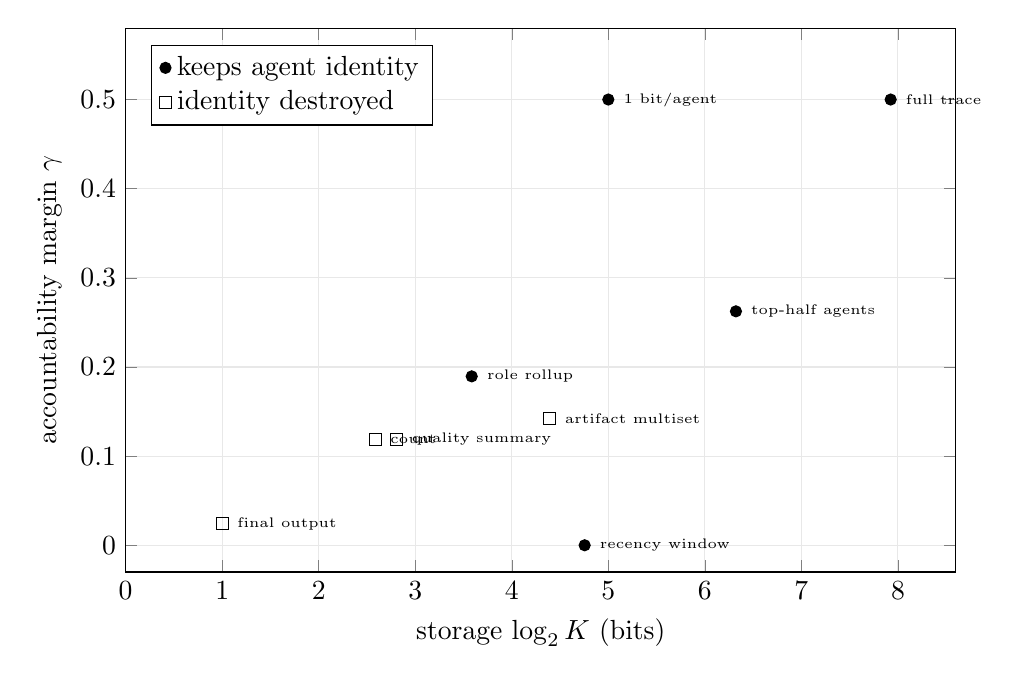
\begin{tikzpicture}
\begin{axis}[
  width=\columnwidth, height=0.70\columnwidth,
  xlabel={storage $\log_2 K$ (bits)},
  ylabel={accountability margin $\gamma$},
  xmin=0, xmax=8.6, ymin=-0.03, ymax=0.58,
  legend pos=north west, legend cell align=left,
  grid=major, grid style={gray!18},
  nodes near coords, point meta=explicit symbolic,
  every node near coord/.append style={font=\tiny, anchor=west, xshift=2pt},
]
\addplot[mark=*, only marks, mark size=2pt] coordinates {(3.5850,0.189474) [role rollup] (4.7549,0.000000) [recency window] (5.0000,0.500000) [1 bit/agent] (6.3219,0.262400) [top-half agents] (7.9248,0.500000) [full trace]};
\addlegendentry{keeps agent identity}
\addplot[mark=square, only marks, mark size=2.2pt] coordinates {(1.0000,0.024300) [final output] (2.5850,0.119020) [count] (2.8074,0.119020) [quality summary] (4.3923,0.142510) [artifact multiset]};
\addlegendentry{identity destroyed}
\end{axis}
\end{tikzpicture}
